\documentclass[11pt]{article}
 
\usepackage[margin=.95in]{geometry} 
\usepackage{amsmath,amsthm,amssymb, graphicx, multicol, array}
 
\newcommand{\N}{\mathbb{N}}
\newcommand{\Z}{\mathbb{Z}}
 

\begin{document}
 
\title{Homework 5}
\author{Juliette Franqueville\\
}
\maketitle

\subsection*{(1) (a)}


\begin{figure}[!h]
    \centering
    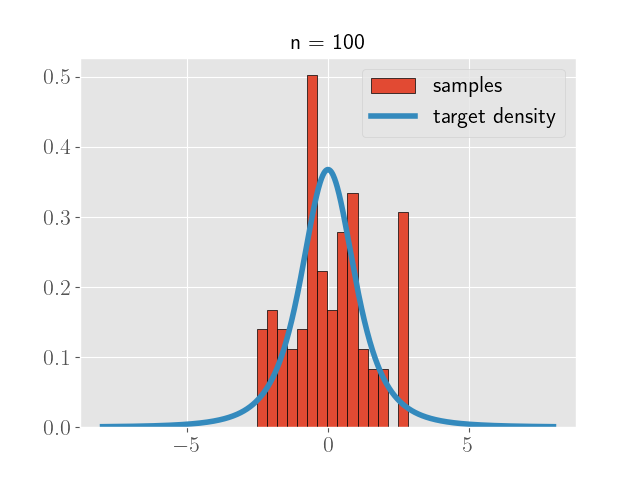
\includegraphics[scale=.6
    ]{../figures/resamples_n_100.png}
    \caption{samples and t distribution for $n=100$}
    \label{fig:my_label}
\end{figure}
\newpage

\begin{figure}[!h]
    \centering
    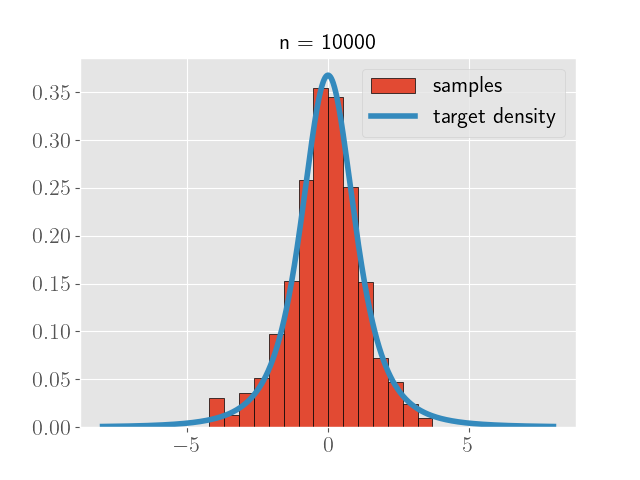
\includegraphics[scale=.6
    ]{../figures/resamples_n_10000.png}
    \caption{samples and t distribution for $n=10,000$}
    \label{fig:my_label}
\end{figure}
\newpage

\subsection*{(2) Consider again a normal likelihood model but with NIP $p(\mu, \sigma^2) \propto \sigma^{-2}$.}



\subsection*{(a) Show that a-posteriori $\mu$ and $\sigma^2$ are dependent but uncorrelated.}



This is essentially the same question as earlier. They are dependent because $\sigma^2$ appears in the pdf of $\mu$. For the posterior of $\sigma^2$, let $\alpha = n/2$ and $\beta = 1/2[(n-1)s^2 + n(\mu - \bar{y})^2]$ in $IG(
\alpha, \beta)$

\begin{align*}
    cov(\mu, \sigma^2|y) &= E(\mu \cdot \sigma^2|y) -  E(\mu|y)E(\sigma^2|y)\\
    &= E_{\sigma^2}E_{\mu|\sigma^2}(\mu \cdot \sigma^2|\sigma^2, y) -  E(\mu|y)E(\sigma^2|y)\\
    &=\bar{y} E_{\sigma^2}  (\sigma^2|y) - \bar{y}\beta/(\alpha - 1)\\
    &= \bar{y}\beta/(\alpha - 1) - \bar{y}\beta/(\alpha - 1) = 0
\end{align*}

\subsection*{(b) Find out the marginal posteriors $p(\mu |y_{1:n})$ and $p(\sigma^2 |y_{1:n})$.}

We use the joint density and integrate w.r.t $\mu$ and $\sigma^2$.
\begin{align*}
    P(\sigma^2|y) &\propto \int P(\sigma^2, \mu|y)d\mu \\
    &\propto \int P(\sigma^2, \mu|y)d\mu \\
    &\propto \int \sigma^{-(n/2 + 1)}e^{\frac{-1}{2\sigma^2}[(n-1)s^2+n(\mu-\bar{y})^2]}d\mu \\
    &\propto \sigma^{-(n/2 + 1)}e^{\frac{-1}{2\sigma^2}(n-1)s^2} \int e^{\frac{-1}{2\sigma^2}[n(\mu-\bar{y})^2]}d\mu \\
     &\propto \sigma^{-(n/2 + 1)}e^{\frac{-1}{2\sigma^2}[(n-1)s^2} (\sigma^2)^{1/2} \\
     &\propto \sigma^{-\left(\frac{n-1}{2}\right)- 1}e^{\frac{-1}{2\sigma^2}(n-1)s^2}\\
     &= IG\left( \frac{n-1}{2}, \frac{1}{2}(n-1)s^2\right)
\end{align*}


\begin{align*}
    P(\mu|y) &\propto \int P(\sigma^2, \mu|y)d\sigma^2 \\
    &\propto \int P(\sigma^2, \mu|y)d\sigma^2 \\
    &\propto \int \sigma^{-(n/2 + 1)}e^{\frac{-1}{2\sigma^2}[(n-1)s^2+n(\mu-\bar{y})^2]}\\
    &\propto [(n-1)s^2+n(\mu-\bar{y})^2]^{-n/2}\\
    &\propto [1+n(\mu-\bar{y})^2/(n-1)s^2]^{-n/2}\\
    &= t_{n-1}(\bar{y}, s^2/n)
\end{align*}


\subsection*{(b) (c) Find out the predictive distribution $p(y_{new} |y_{1:n})$.}

\begin{align*}
    p(y_{new} |y_{1:n}) &= \int \int p(y_{new} |y_{1:n}, \sigma^2, \mu)P(\mu, \sigma^2|y)d\mu d\sigma^2\\
     &= \int \int p(y_{new} |y_{1:n}, \sigma^2, \mu)P(\mu| \sigma^2,y)P(\sigma^2|y)d\mu d\sigma^2\\
\end{align*}

Take the inner integral first


\begin{align*}
  & \int p(y_{new} |y_{1:n}, \sigma^2, \mu)P(\mu| \sigma^2,y)d\mu \\
  & \int\propto (\sigma^2)^{-1/2}e^{-1/2\sigma^2(y_{new}-\mu)^2}(\sigma^2)^{-1/2}e^{-n/2\sigma^2(\mu-\bar{y})^2}d\mu\\
  & \int\propto (\sigma^2)^{-1}e^{-1/2\sigma^2[(y_{new}-\mu)^2+n(\mu-\bar{y})^2]}d\mu\\
   & \int\propto (\sigma^2)^{-1}e^{-1/2\sigma^2[y_{new}^2-2y_{new}\mu+\mu^2+n\mu^2-2n\mu\bar{y}+n\bar{y}^2]}d\mu\\
      & \int\propto (\sigma^2)^{-1}e^{-1/2\sigma^2[\mu^2(n+1)-2\mu(y_{new}+n\bar{y})+y_{new}^2]}d\mu\\
       & \int\propto (\sigma^2)^{-1}e^{-(n+1)/2\sigma^2[\mu^2-2\mu(y_{new}+n\bar{y})/(n+1)+y_{new}^2/(n+1)]}d\mu\\
       & \int\propto (\sigma^2)^{-1}e^{-(n+1)/2\sigma^2[\{\mu-(y_{new+n\bar{y}}/(n+1)\}^2-\{(y_{new+n\bar{y}}/(n+1)\}^2+y_{new}^2/(n+1)]}d\mu\\
       &\propto (\sigma^2)^{-1}(\sigma^2)^{1/2}e^{-(n+1)/2\sigma^2[-\{(y_{new+n\bar{y}}/(n+1)\}^2+y_{new}^2/(n+1)]}\\
       &\propto (\sigma^2)^{-1/2}e^{-(n+1)(n+1)^{-2}/2\sigma^2[-y_{new}^2-2y_{new}n\bar{y}-n^2\bar{y}^2+y_{new}^2(n+1)]}\\
       &\propto (\sigma^2)^{-1/2}e^{-n(n+1)^{-1}/2\sigma^2[y_{new}^2-2y_{new}\bar{y}]}\\
        &\propto (\sigma^2)^{-1/2}e^{-n(n+1)^{-1}/2\sigma^2[y_{new}^2-\bar{y}]^2}\\
        &\propto \mathcal{N}(\bar{y}, (n+1)\sigma^2/n )
\end{align*}

Now the full integral

\begin{align*}
    p(y_{new} |y_{1:n}) &\propto 
     \int P(\sigma^2|y)[ (\sigma^2)^{-1/2}e^{-n(n+1)^{-1}/2\sigma^2[y_{new}^2-\bar{y}]^2} d\sigma^2\\
     &  \int \propto  \sigma^{-\left(\frac{n-1}{2}\right)- 1}e^{\frac{-1}{2\sigma^2}(n-1)s^2} e^{-n(n+1)^{-1}/2\sigma^2[y_{new}^2-\bar{y}]^2} d\sigma^2\\
      &  \int \propto  \sigma^{-n/2-1}e^{\frac{-1}{2\sigma^2}[(n-1)s^2 + n/(n+1)(y_{new}^2-\bar{y})^2]}  d\sigma^2\\
      & \propto [(n-1)s^2 + n/(n+1)(y_{new}^2-\bar{y})^2] ^{-n/2} \int IG(n/2, 1/2 [(n-1)s^2 + n/(n+1)(y_{new}^2-\bar{y})^2])d\sigma^2\\
      &\propto [(n-1)s^2 + n/(n+1)(y_{new}^2-\bar{y})^2] ^{-n/2}\\
       &\propto [1 + n/(n+1)(y_{new}^2-\bar{y})^2/(n-1)s^2] ^{-n/2}\\
       &= t_{n-1}(\bar{y}, (n+1) s^2/n)
\end{align*}

f

\subsection*{(3) For a multinomial likelihood model with K categories, show that the Jeffreys’ prior for the category probabilities is $Dir(1/2, \ldots, 1/2)$.}

For the multinomial distribution:

\begin{align*}
   \mathcal{L}(y_1, \ldots y_k| n, p_1 \ldots p_k) &= \text{log} \frac{n}{x_1! \ldots x_k!} \prod p_i^{x_i}\\
   &= \text{log} \frac{n}{x_1! \ldots x_k!}  + \sum \text{log} p_i^{x_i}
\end{align*}


\begin{align*}
   \frac{\partial}{\partial p_i}\mathcal{L}(y_1, \ldots y_k| n, p_1 \ldots p_k) 
   &=   \frac{x_i}{p_i}\\
   \frac{\partial^2}{\partial p_i \partial p_j}\mathcal{L}(y_1, \ldots y_k| n, p_1 \ldots p_k) &= \begin{cases}
  -\frac{x_i}{p_i^2},  &  i = j \\
  0, & \text{otherwise}
\end{cases}
\end{align*}

In order words, this is a $k$ by $k$ diagonal matrix with diagonal elements $ -x_i/p_i^2$. We also have $-E(-x_i/p_i^2)  = E(x_i)/p_i^2 = n p_i/p_i^2 = n/p_i$, so the information matrix is

\begin{align*}
    I(p_1, \dots, p_k) &=  \begin{bmatrix}
    n/p_1 & & \\
    & \ddots & \\
    & & n/p_k
  \end{bmatrix}
\end{align*}

and Jeffreys prior is:

\begin{align*}
    p_1, 
    \ldots, p_n&\propto \text{det}\begin{bmatrix}
    n/p_1 & & \\
    & \ddots & \\
    & & n/p_k
  \end{bmatrix}^{1/2}\\
  &\propto \prod p_k^{-1/2}\\
  &\propto \prod p_k^{1/2-1}\\
  &\propto Dir(1/2, \dots 1/2)
\end{align*}

\subsection*{(4) (a) Using the EM algorithm, fit location mixtures of normals to the Galaxy data.}

\begin{figure}[!h]
    \centering
    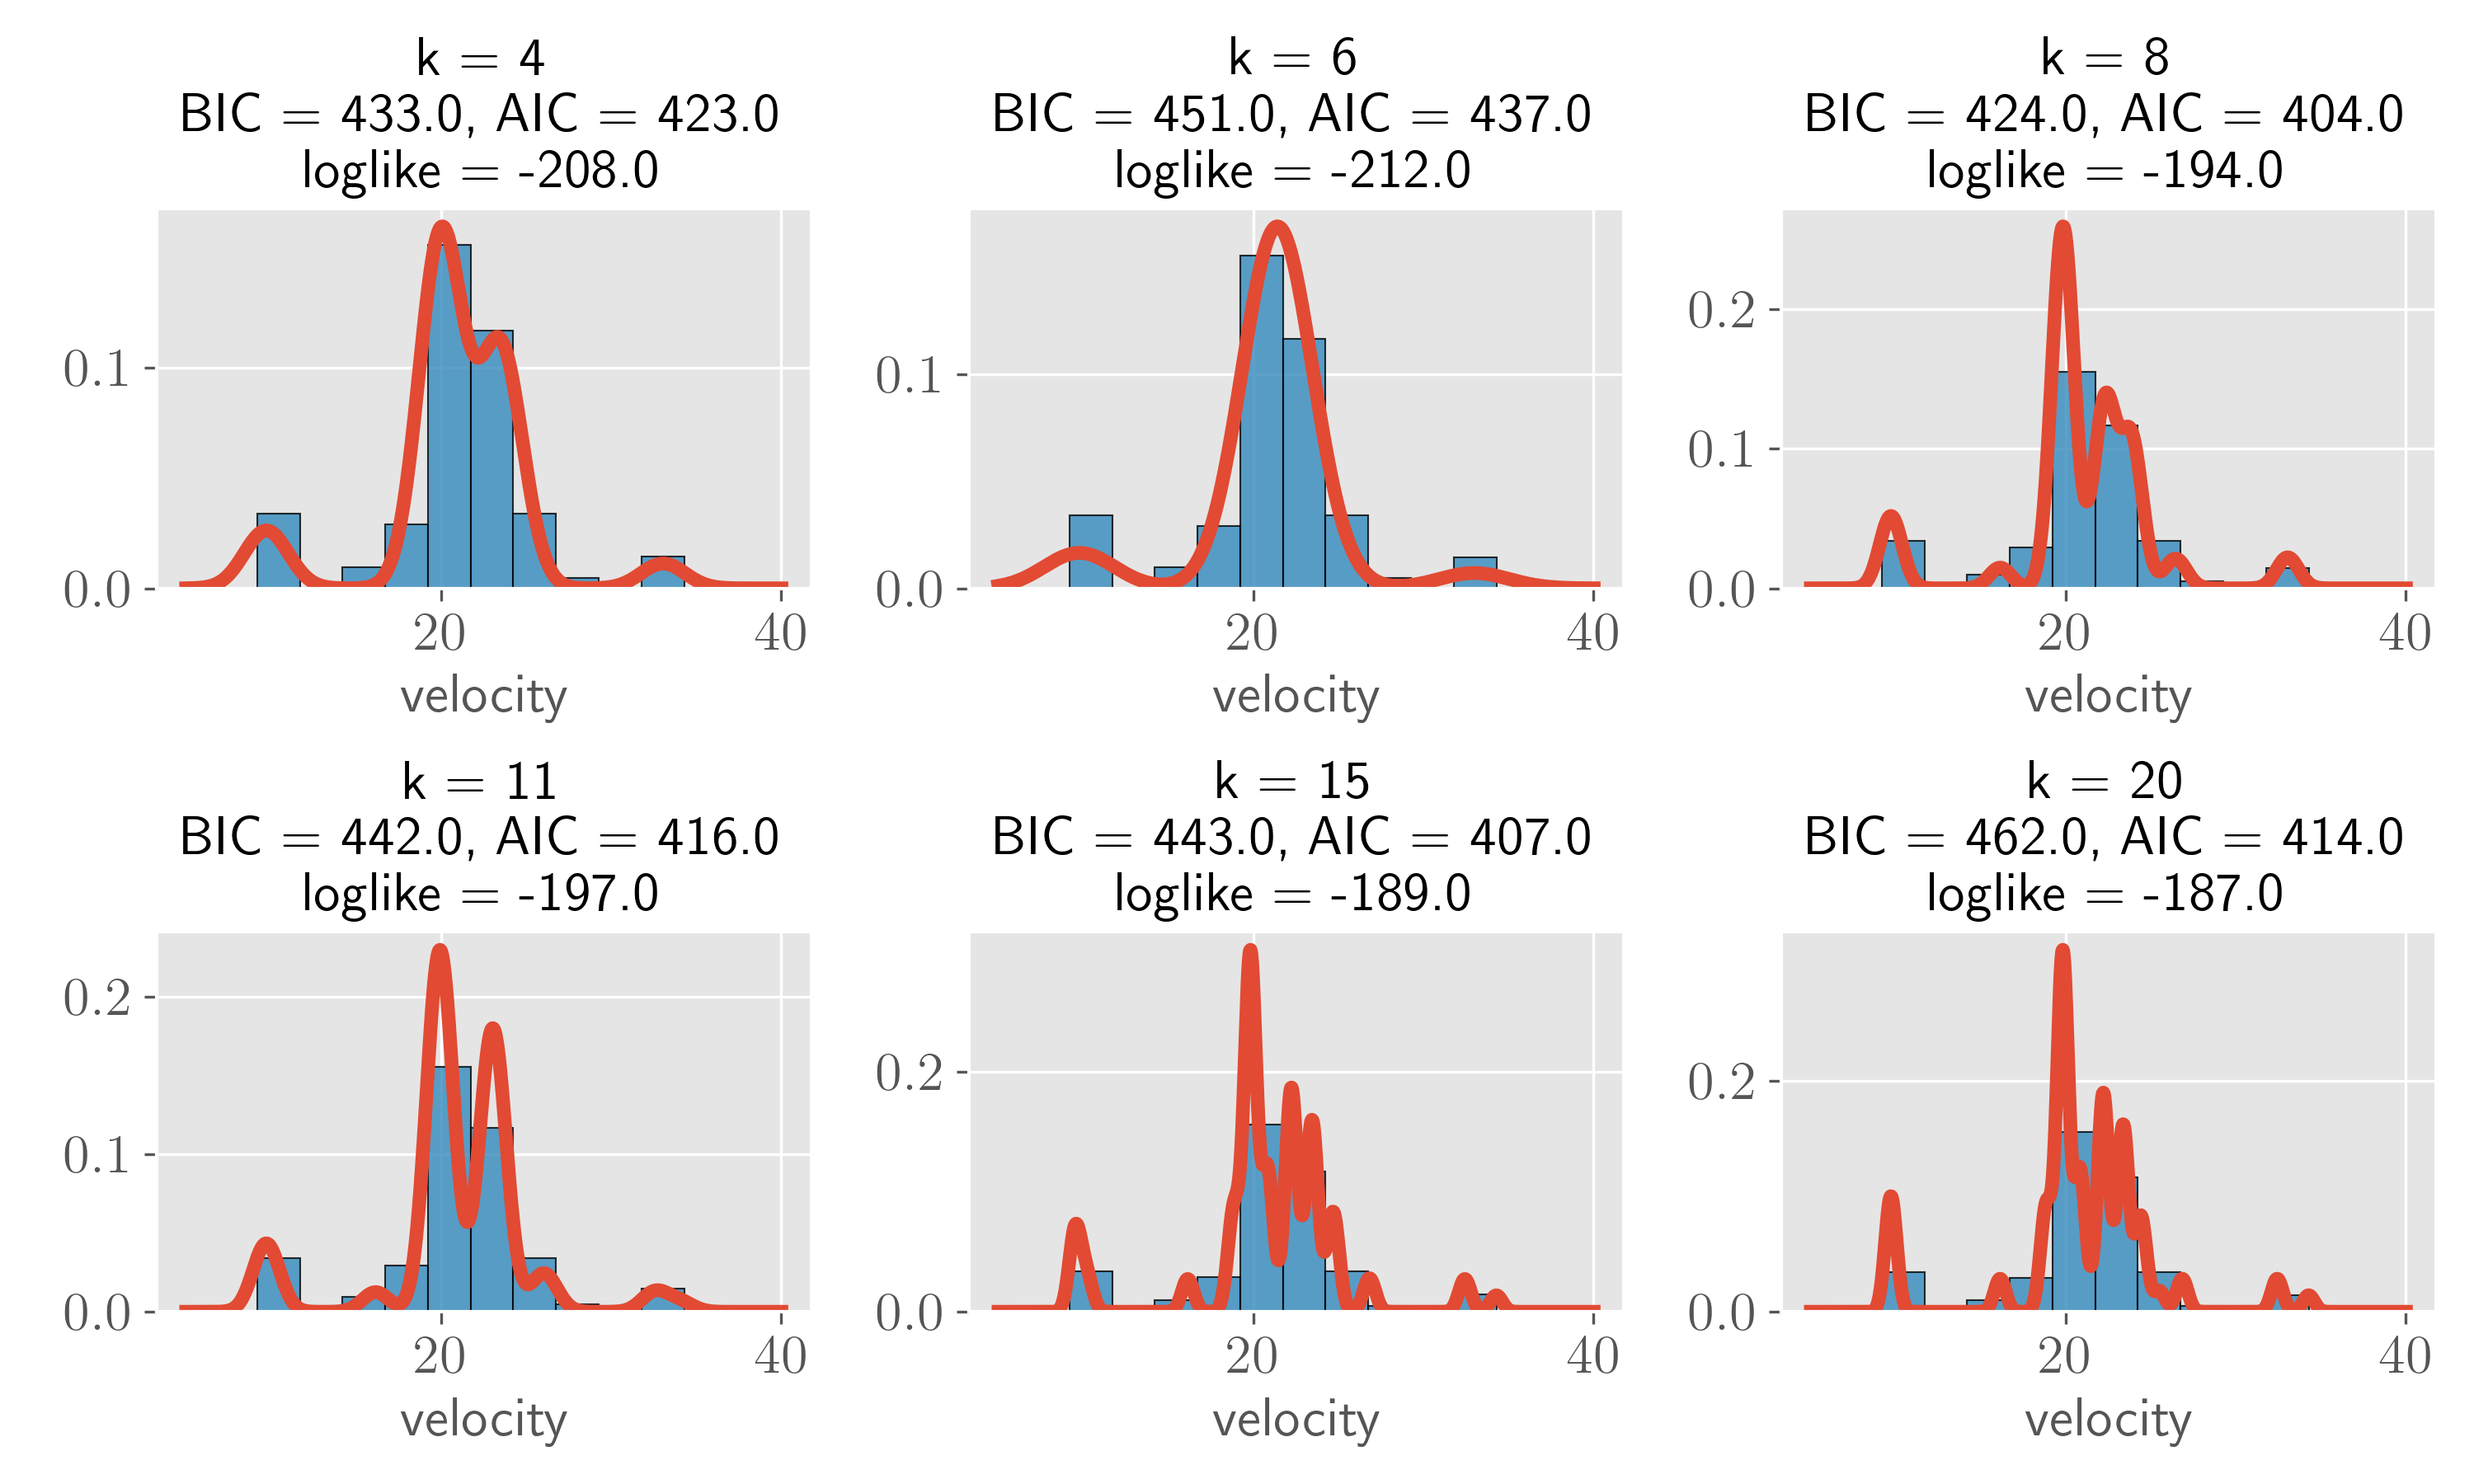
\includegraphics[scale=.6
    ]{homework_4/figures/galaxies_1.png}
    \caption{Results when the variances and pooled.}
    \label{fig:my_label}
\end{figure}
\newpage

\subsection*{(b) Tabulate AIC and BIC values for each case and report the ‘best’ model(s)}

The AIC and BIC values are shown on the plots. $k =8$ has both the lowest BIC and AIC.

\subsection*{(c) Next, fit location-scale mixtures of normals [where the variances are not pooled]}

\begin{figure}[!h]
    \centering
    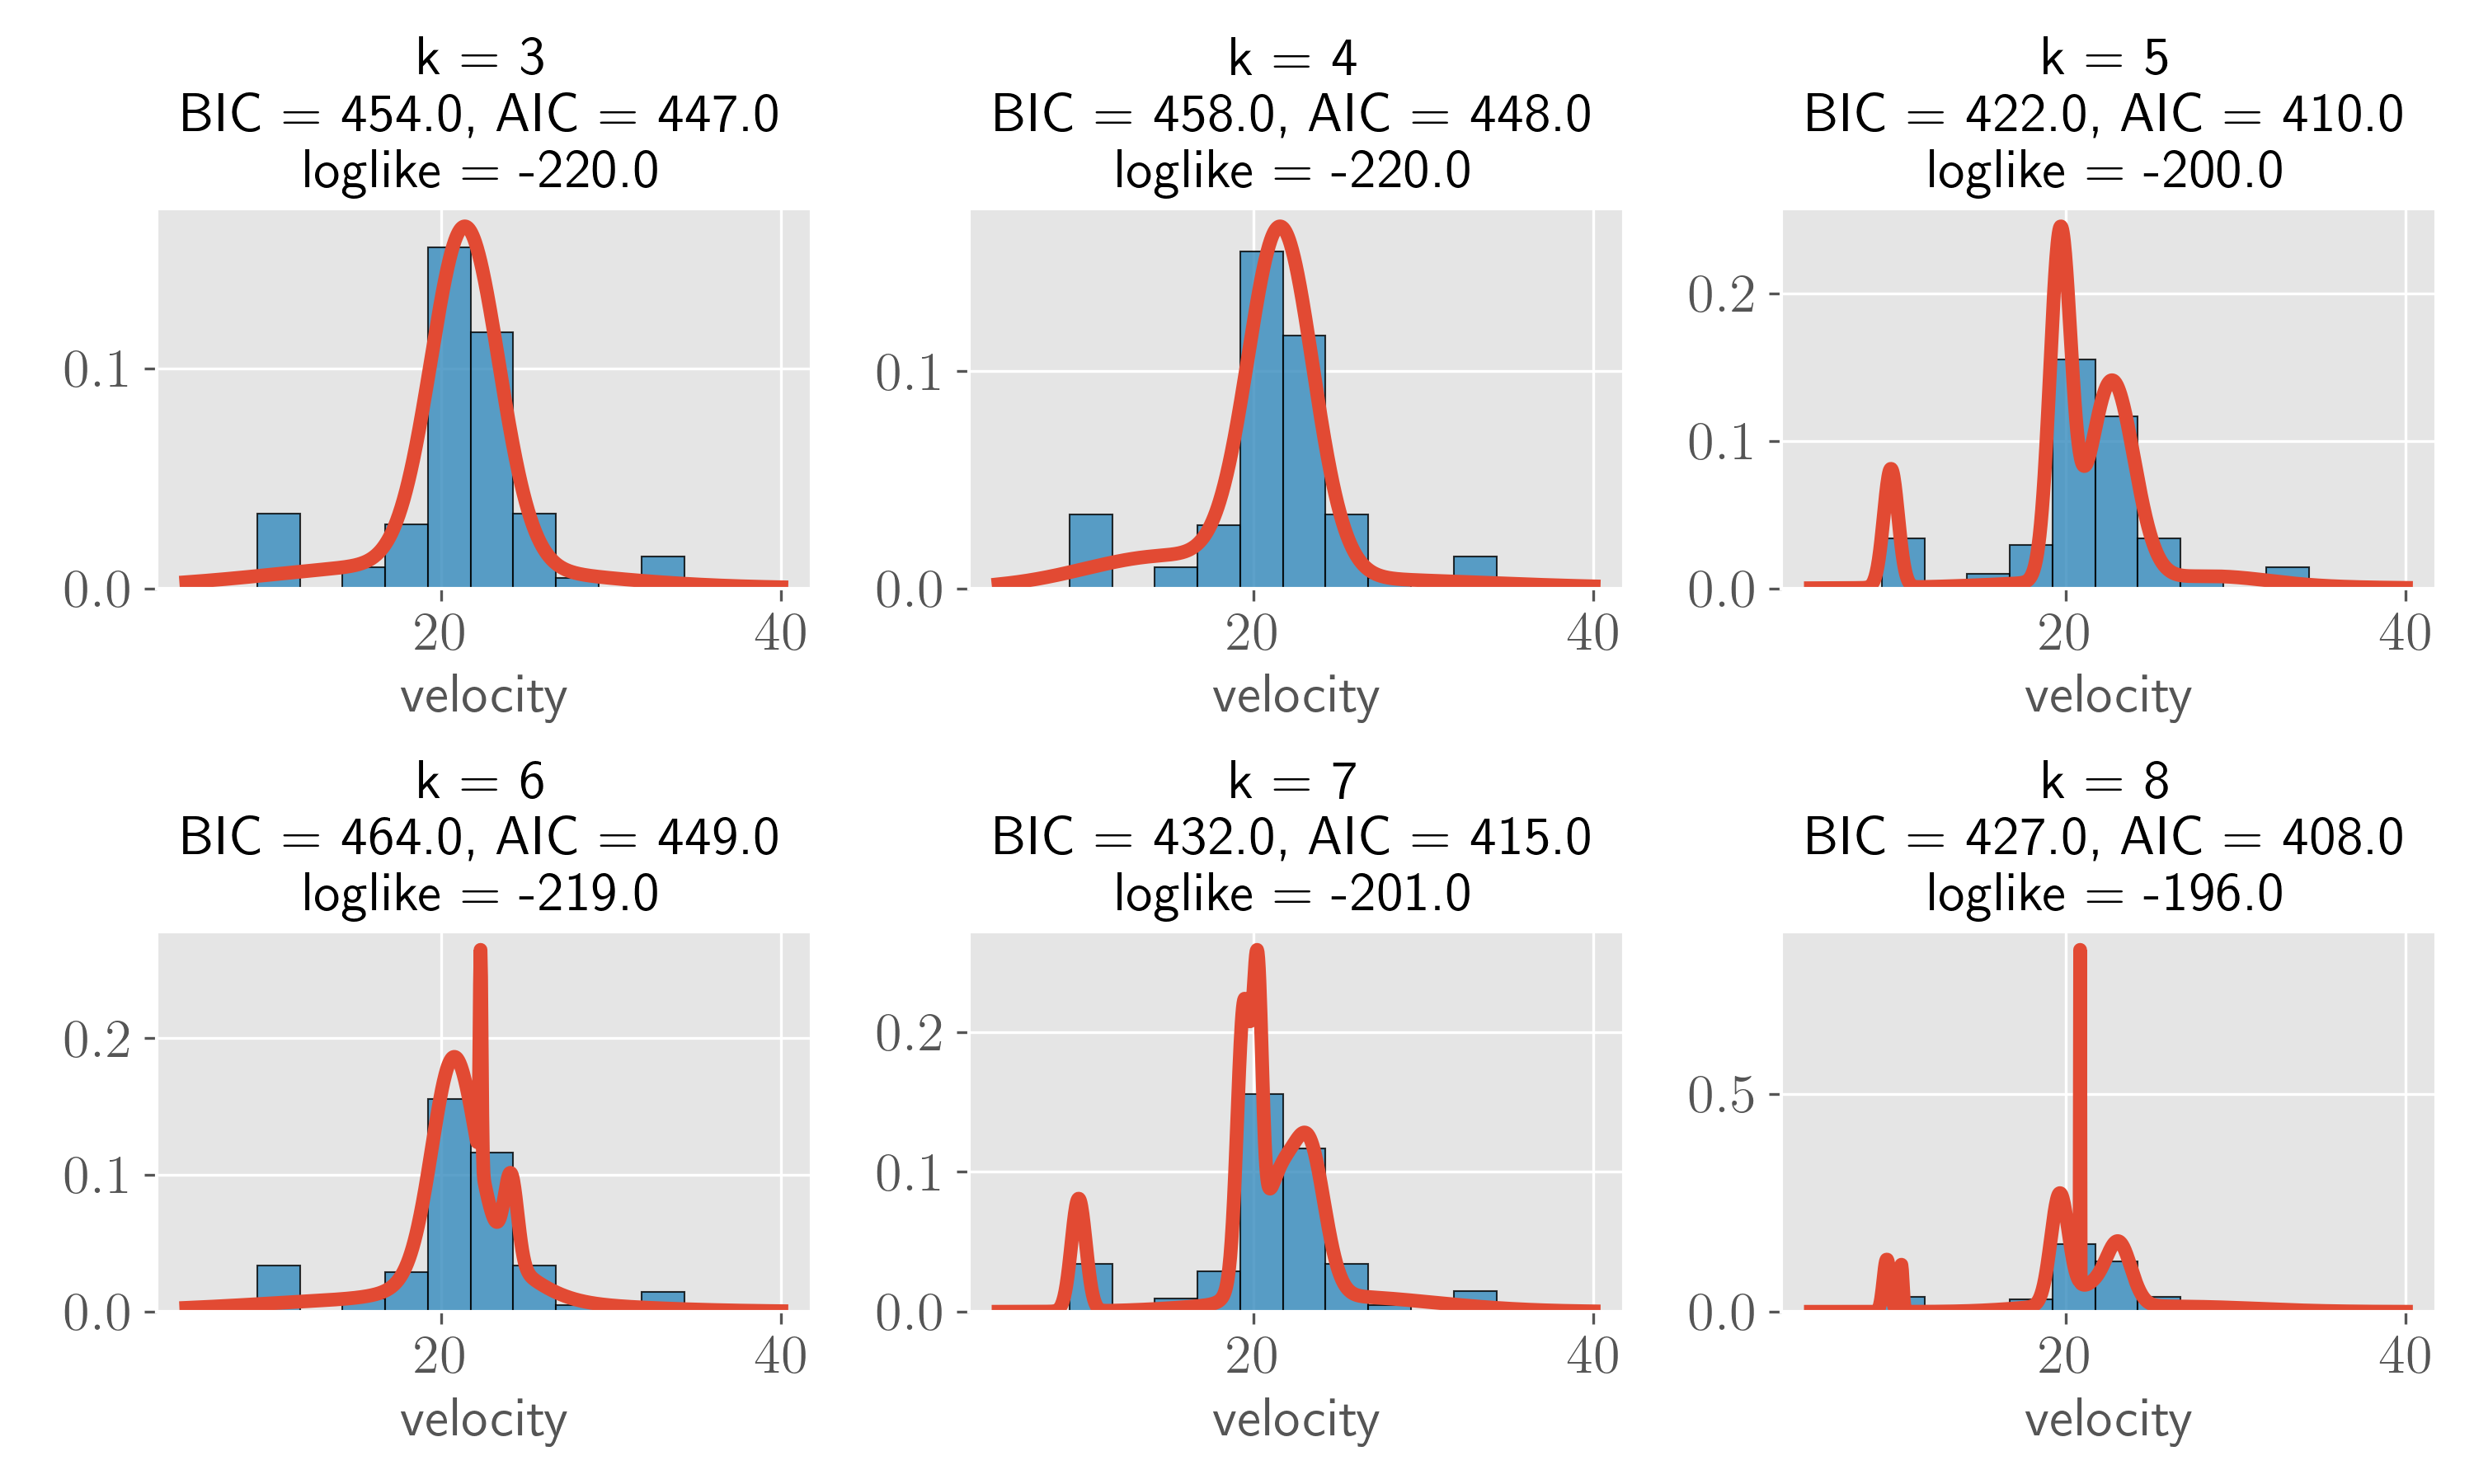
\includegraphics[scale=.6
    ]{homework_4/figures/galaxies_2.png}
    \caption{Results when the variances and not pooled ($k$ variances).}
    \label{fig:my_label}
\end{figure}

\newpage
\subsection*{(d) Tabulate AIC and BIC values for each case and report the ‘best’ model(s)}

The AIC and BIC values are shown on the plots. $k =5$ had the lowest BIC but $k=8$ has the lowest AIC.


\subsection*{(e) Summarize your general findings}
As expected, increasing the number of $k$ generally increases the likelihood of the data, but can cause overfitting. The AIC and BIC measures take this into account by penalizing model complexity. Having a different variance for each normal allows for more flexibility in the model. The results seemed very dependent on starting conditions.

\subsection*{(5) Repeat everything you did in Problem No 3 above but this time using the stochastic EM algorithm}

\subsection*{ (a) Using the EM algorithm, fit location mixtures of normals to the Galaxy data}

\begin{figure}[!h]
    \centering
    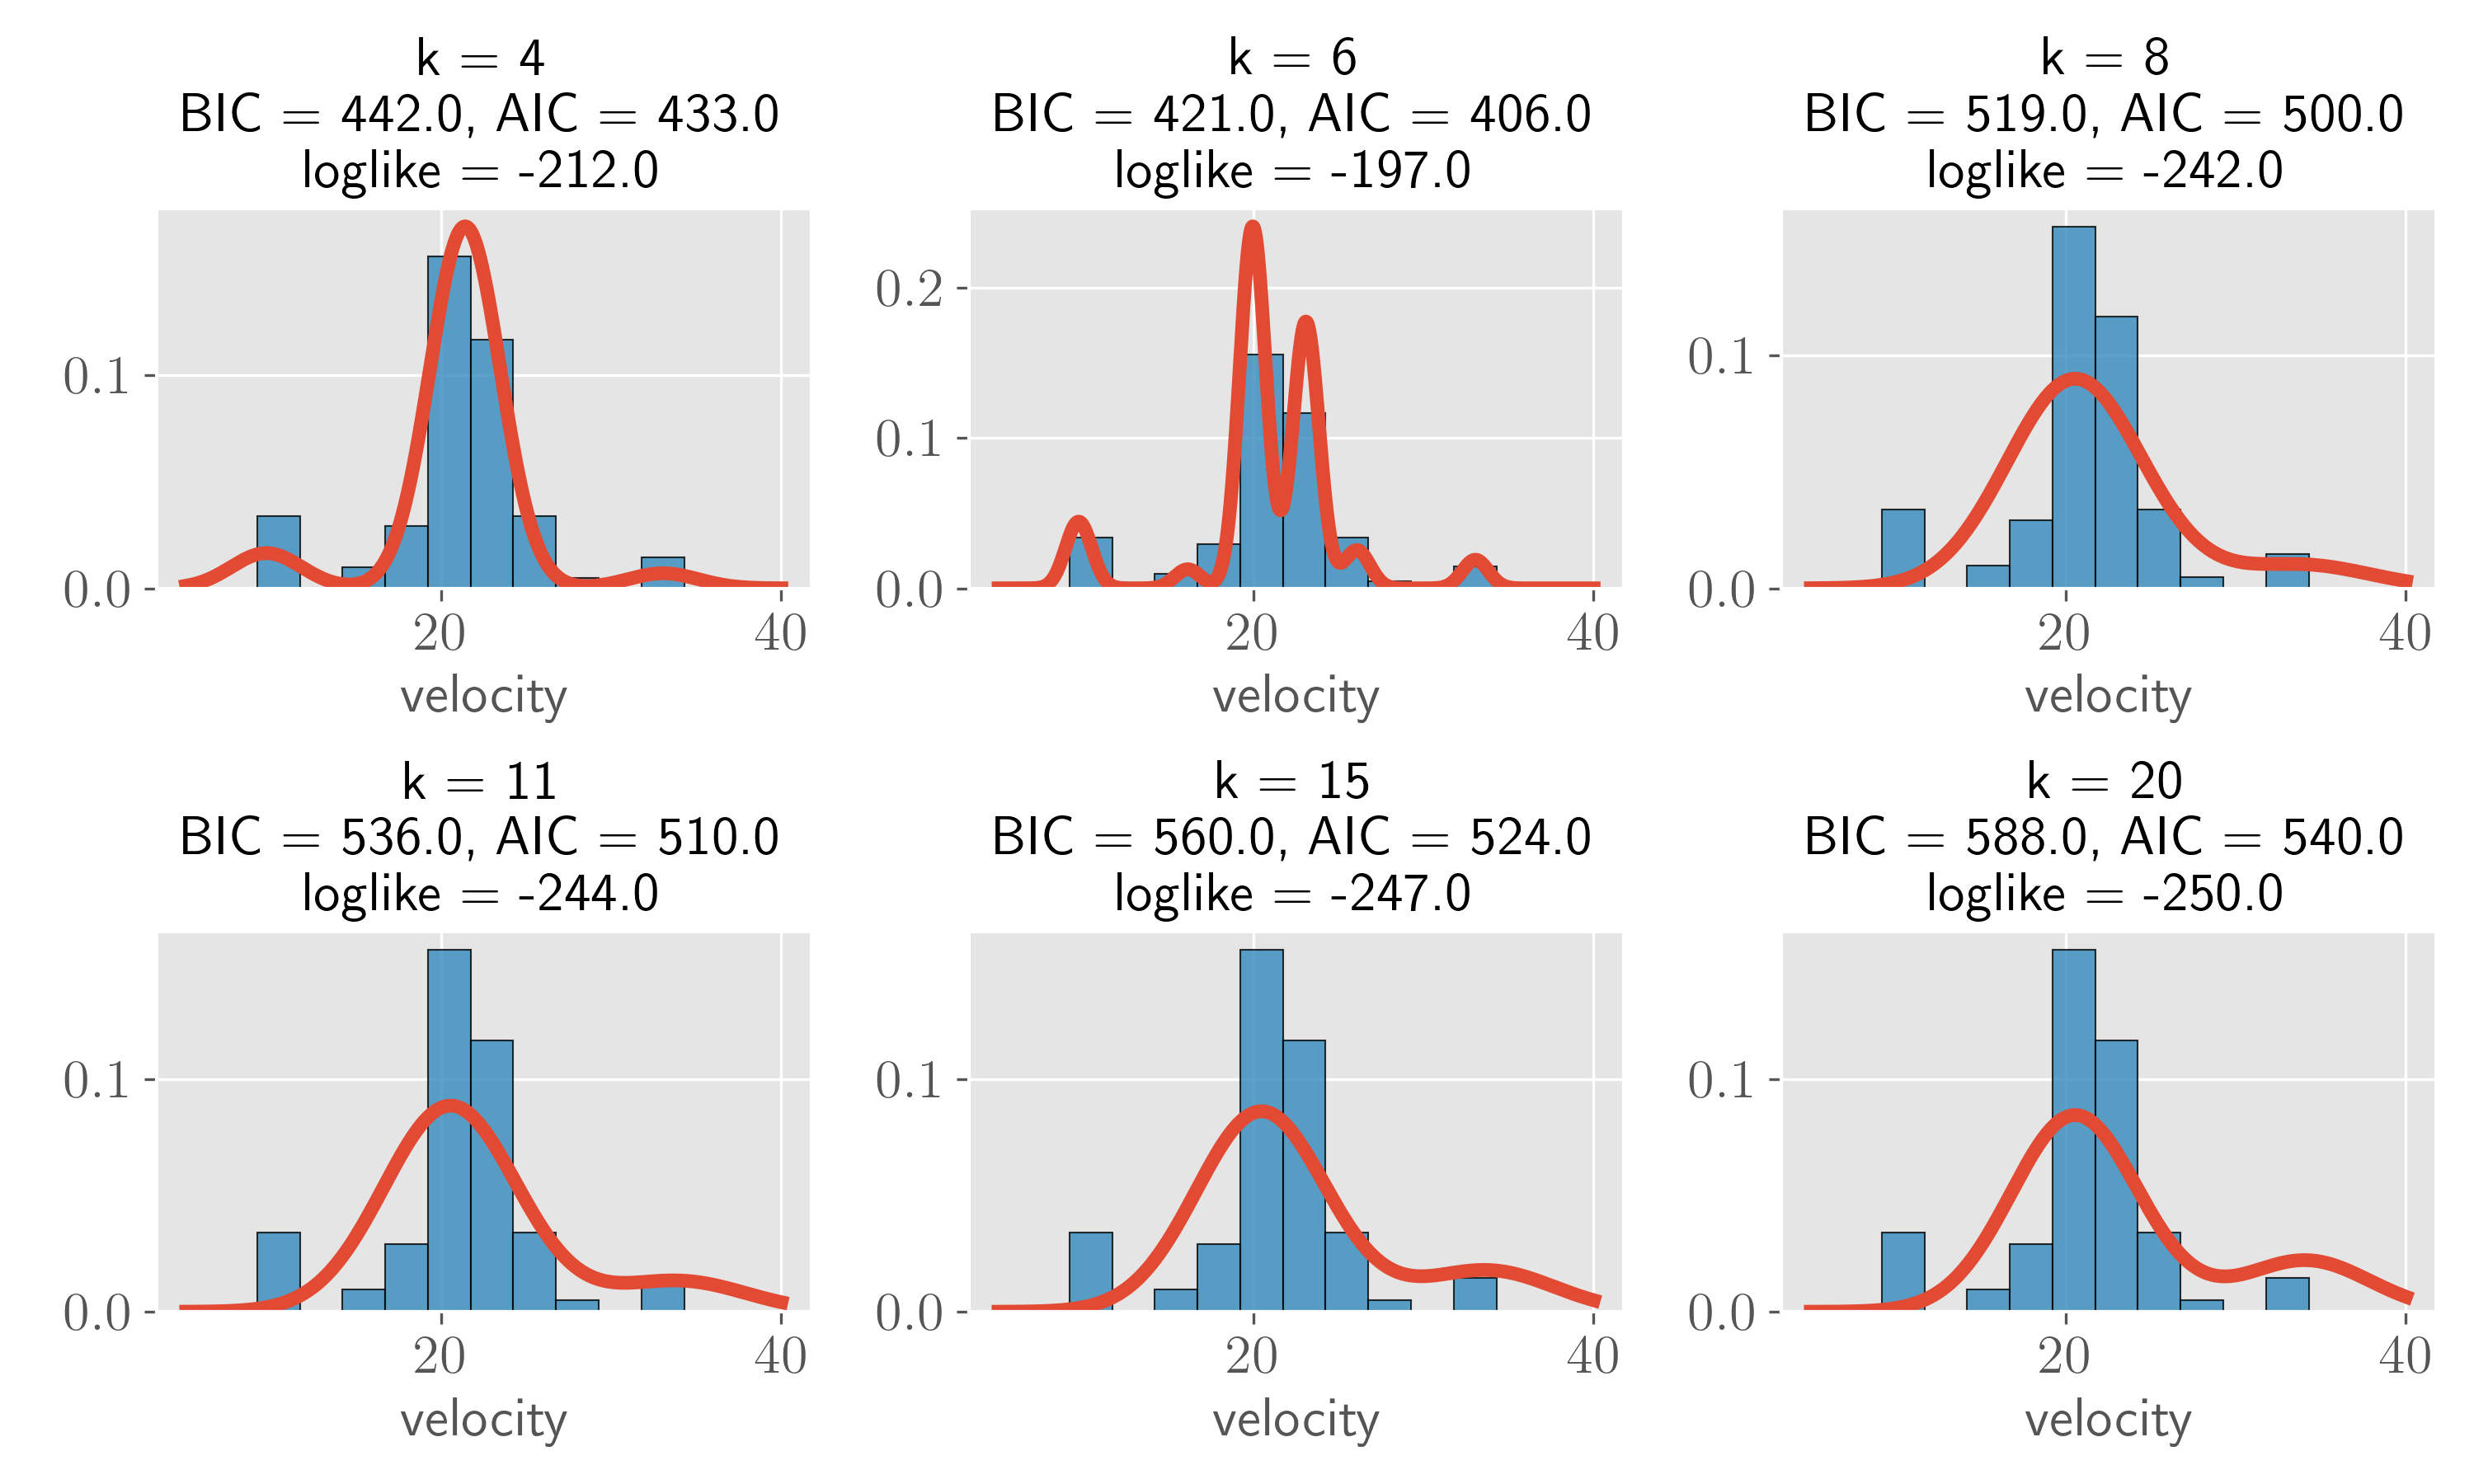
\includegraphics[scale=.6
    ]{homework_4/figures/galaxies_3.png}
    \caption{Results when the variances and pooled, stochastic.}
    \label{fig:my_label}
\end{figure}
\newpage

\subsection*{ (b) Tabulate AIC and BIC values for each case and report the ‘best’ model(s)}

The AIC and BIC values are shown on the plots. $k=6$ has the lowest BIC and AIC.

\subsection*{(c) Next, fit location-scale mixtures of normals [where the variances are not pooled]}

\begin{figure}[!h]
    \centering
    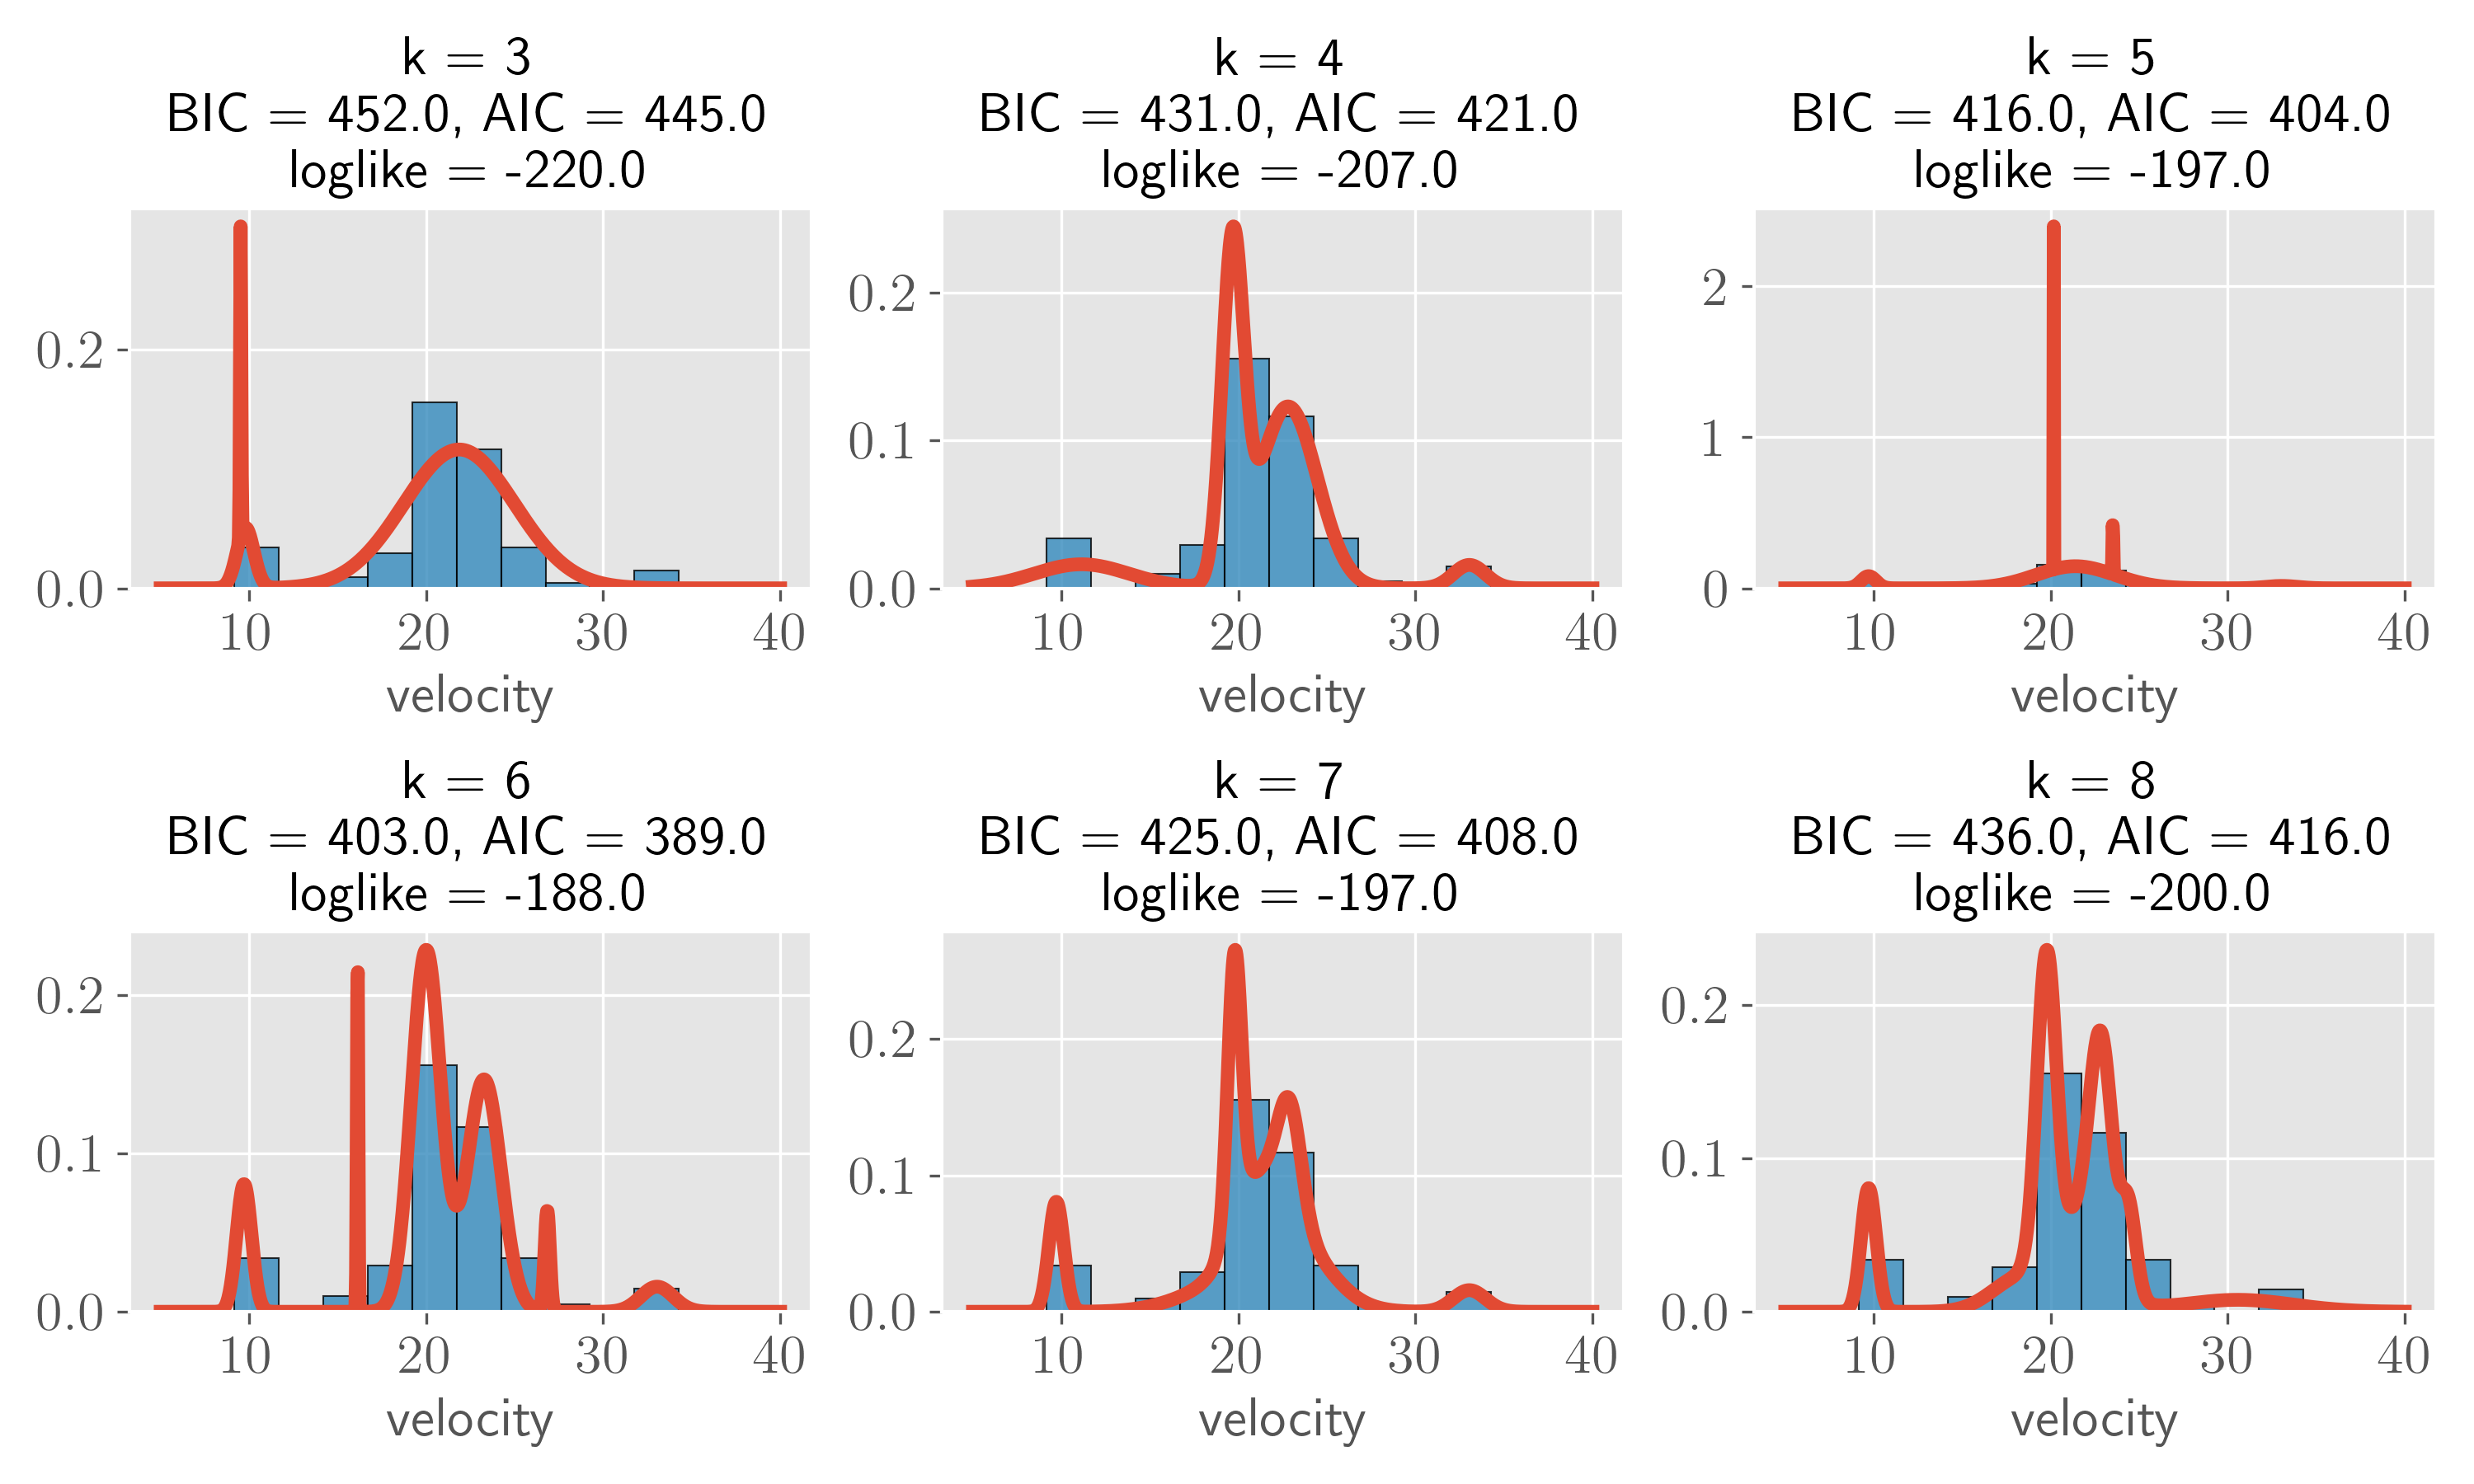
\includegraphics[scale=.6
    ]{homework_4/figures/galaxies_4.png}
    \caption{Results when the variances and not pooled ($k$ variances), stochastic.}
    \label{fig:my_label}
\end{figure}
\newpage
\subsection*{(d) Tabulate AIC and BIC values for each case and report the ‘best’ model(s).}

The AIC and BIC values are shown on the plots. $k=6$ had the lowest BIC and $k=6$ had the lowest AIC.

\subsection*{(e) Summarize your general findings}
The conclusions are similar as before; increasing the number of $k$ generally increases the likelihood of the data, but can cause overfitting.  I found it more difficult to get the stochastic EM algorithms to converge. In fact, I am not sure that the algorithm converged for all $k$ values in the case where the variances were all the same. As before, the results seemed very dependent on starting conditions. With the stochastic method, I was not sure how to deal with the fact that there was no guarantee that all $k$ would be sampled in $z_i \sim Mult(1, \pi_i)$. I made sure it was the case by sampling again if a $k$ had not been sampled, but this made the algorithm slower.




\subsection*{(6) The ‘faithful’ dataset from package ‘datasets’ in R gives eruption and waiting times of the old faithful geyser in Yellowstone national park (export this dataset from R if you are using a different programming language)}

\subsection*{(a) Using the EM algorithm, fit location-scale mixtures of bivariate normals}
\begin{figure}[!h]
    \centering
    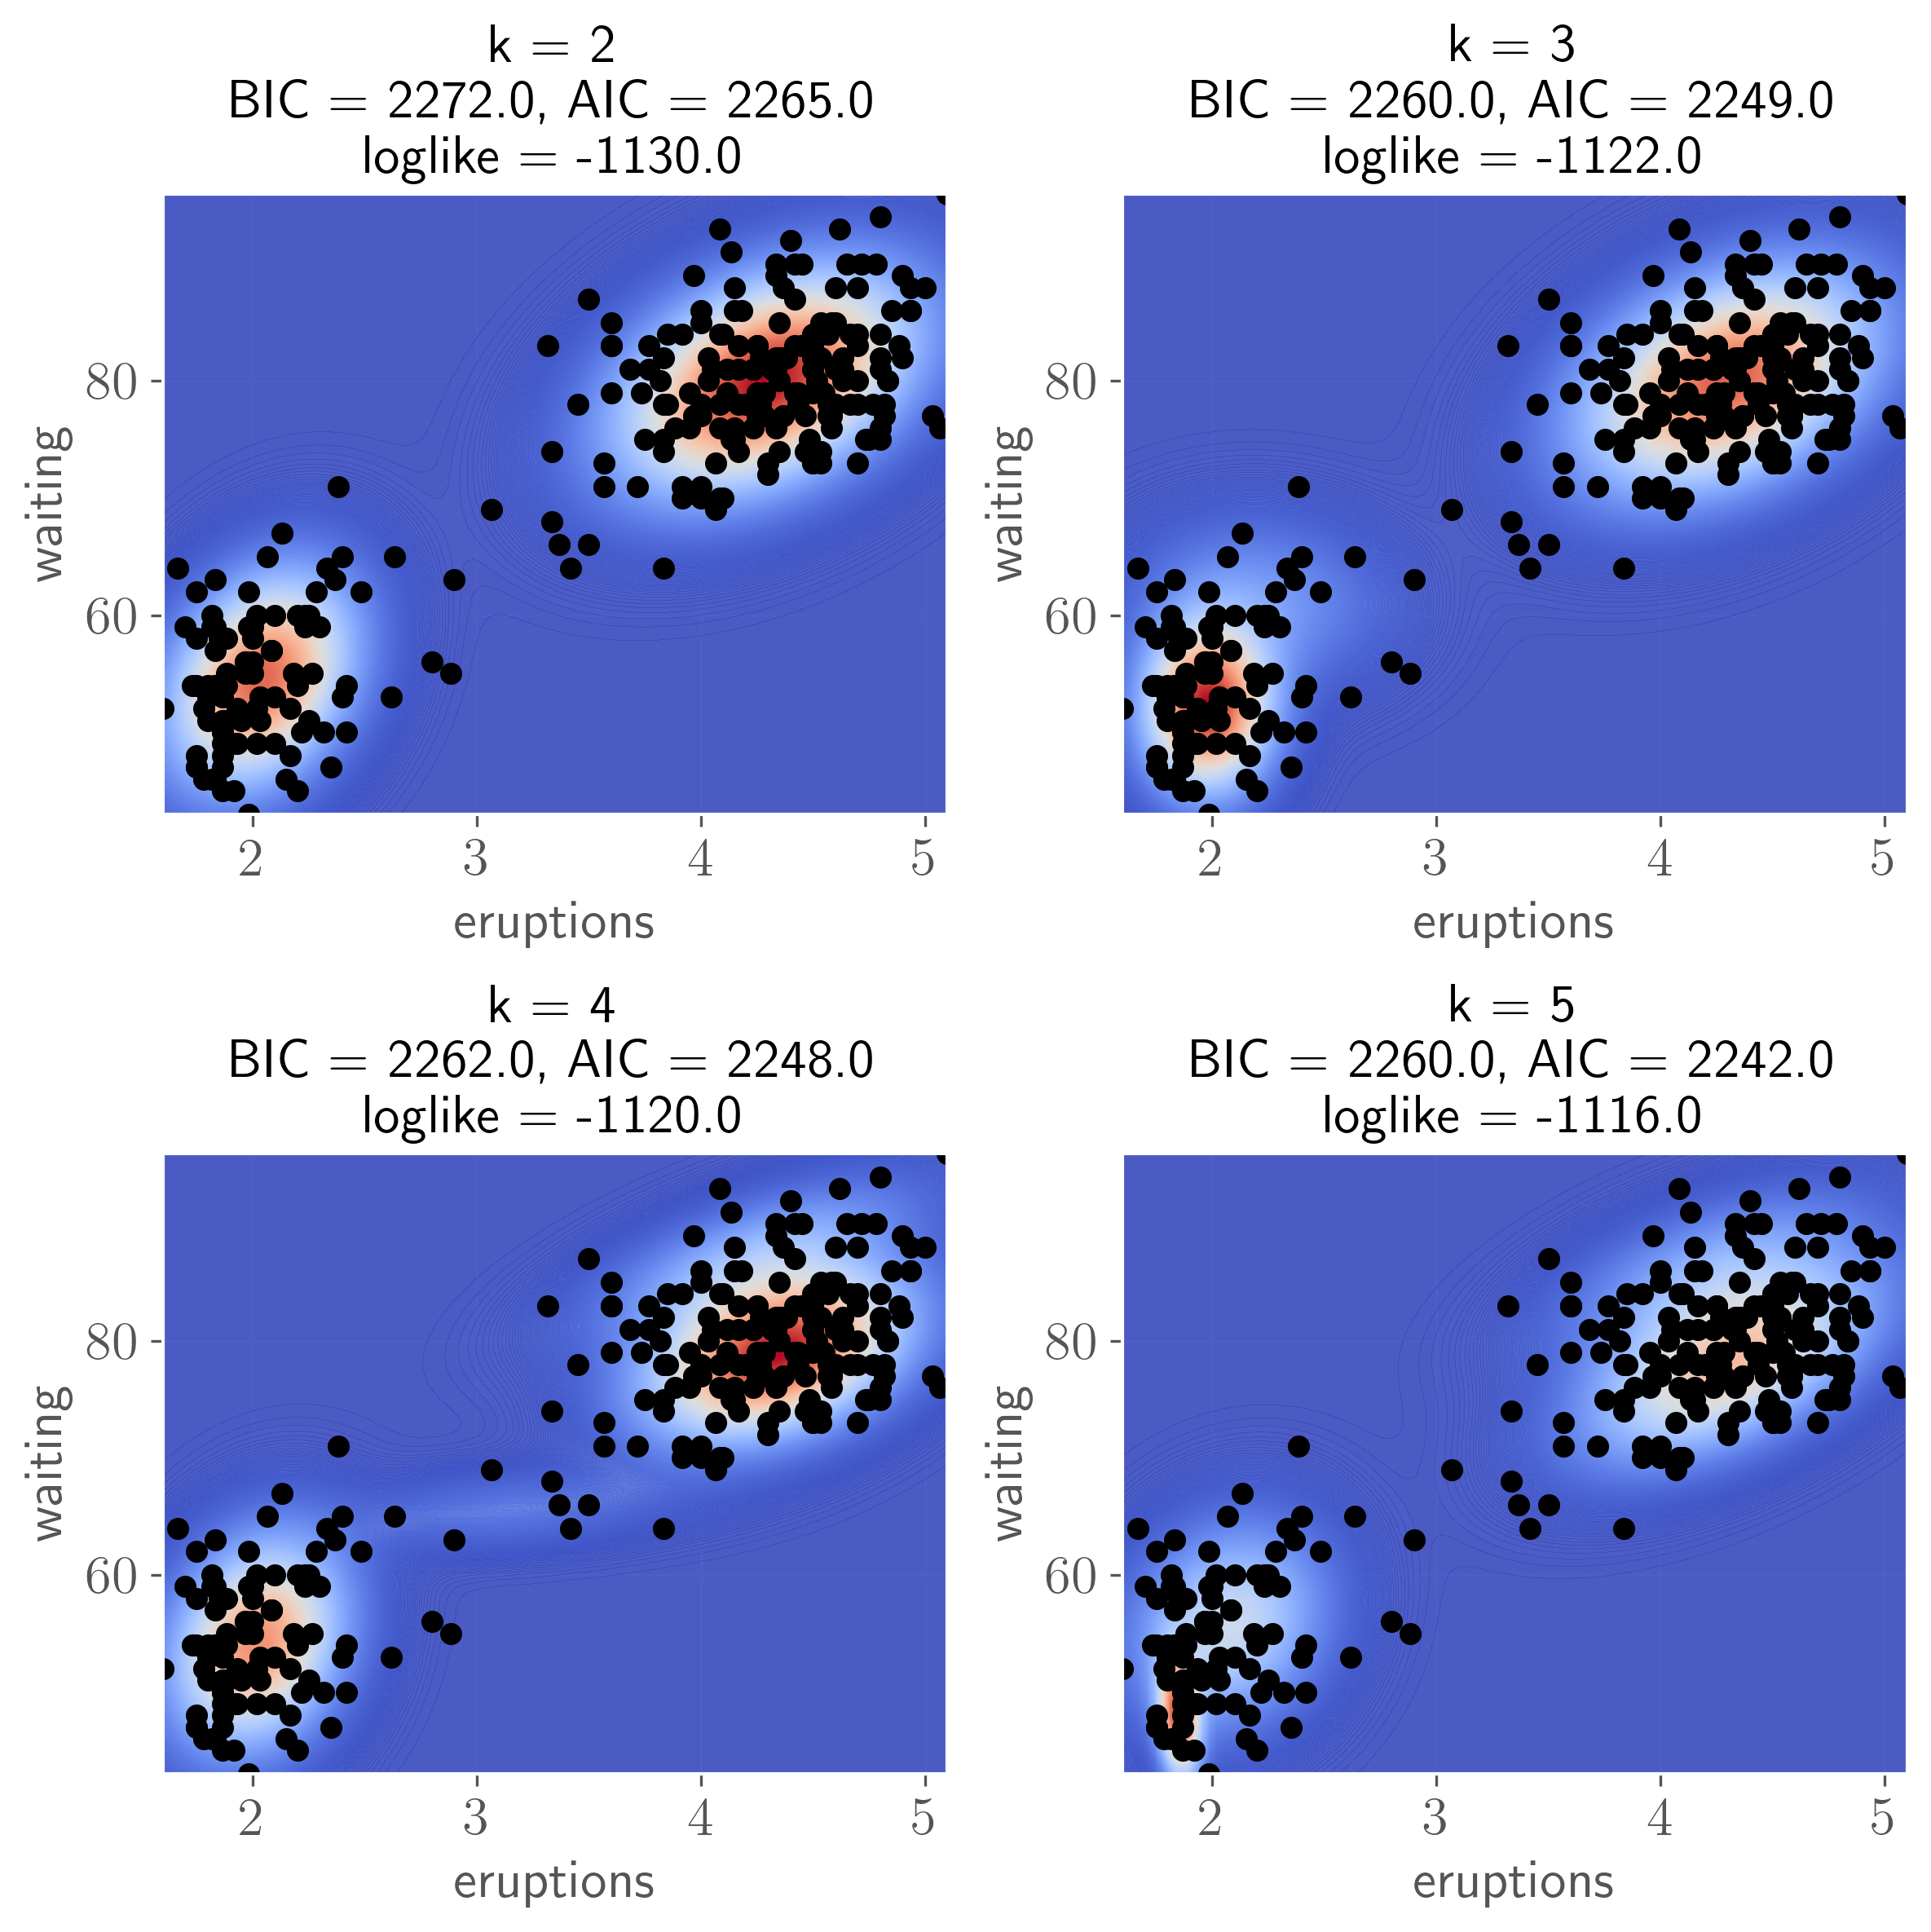
\includegraphics[scale=.6
    ]{homework_4/figures/bivariate.png}
    \caption{Results for $k$ bivariates. Note that some of the bivariates have means close to each other, so it is difficult to distinguish them from the plots.}
    \label{fig:my_label}
\end{figure}
\newpage
\subsection*{(b) Tabulate AIC and BIC values for each case and report the ‘best’ model(s).}
The values are shown in the plot. $k=5$ had the lowest BIC and AIC values, though they were very close to those for $k=3, 4$. As before, I had trouble getting the algorithm to converge and it took many attempts with different starting values to obtain reasonable results.



\end{document}
